%Here is the method used to examine the question
In this chapter, the methods employed to answer the proposed question are presented. This chapter begins by establishing the data sets and data processing utilized in this project. Thereafter relevant neural network architectures are outlined. Finally, the approaches for training the generative models are presented. Three approaches of this kind have been employed in this project: standard \acrshort{vaes}, progressive \acrshort{gans} and Autoencoding \acrshort{gans}. They are presented in their respective section.

\section{Synthetic Data Sets}
The initial experiments in this study are performed on synthetic data obtained through rendering of a 3D head model in a data generation framework. This framework is based on the work of \textcite{swirski2014rendering} and utilizes the same head rig. Two data sets with resolution 256x256 was generated. For reproducability, the data sets will become publicly available at the time of publication.

The synthetic data sets are fully annotated with automatically generated ground truth labels. The relevant labels for the experiments are converted to heatmaps when loaded for training and evaluation as in most cases of semantic segmentation \parencite{guo2017review}. These heatmaps are thereafter concatenated with the real images, forming feature maps of shape 2x320x320. By viewing the annotations as a part of the data, unsupervised models that learn the data distribution implicitly learn the relations between the annotations and the images.

\section{Network architectures}
...relevant network architectures are described here, together with figures and stuff. Base it around GAN networks, the small differences in the encoders can be explained afterwards.

\begin{table}[t]
    \centering
    \caption{Generator architecture used in the experiments. Feature normalization and leaky ReLUs were applied after each convolution except}
    \label{tab:generator}
    \begin{tabular}{lll}
        \hline
        %\multicolumn{3}{c}{Generator}           \\ 
        Operation          & Shape     & Stride \\ \hline
        Input              & 128x1x1   & 1      \\
        Conv 4x4           & 128x4x4   & 1      \\
        Conv 3x3           & 128x4x4   & 1      \\ \hline
        Transpose Conv 2x2 & 128x8x8   & 2      \\
        Conv 3x3           & 112x8x8   & 1      \\ \hline
        Transpose Conv 2x2 & 11216x16   & 2      \\
        Conv 3x3           & 96x16x16   & 1      \\ \hline
        Transpose Conv 2x2 & 96x32x32   & 2      \\
        Conv 3x3           & 80x32x32   & 1      \\ \hline
        Transpose Conv 2x2 & 80x64x64   & 2      \\
        Conv 3x3           & 64x64x64   & 1      \\ \hline
        Transpose Conv 2x2 & 64x128x128   & 2      \\
        Conv 3x3           & 32x128x128   & 1      \\ \hline
        Transpose Conv 2x2 & 32x256x256   & 2      \\
        Conv 3x3           & 16x256x256   & 1      \\ \hline
        Conv 1x1           & 2x256x256 & 1     
    \end{tabular}
\end{table}

\begin{table}[t]
    \centering
    \caption{Discriminator architecture}
    \label{tab:generator}
    \begin{tabular}{lll}
        \hline
        %\multicolumn{3}{c}{Discriminator}           \\ 
        Operation          & Shape     & Stride \\ \hline
        Input              & 2x256x256   & 1   \\
        Conv 1x1           & 16x256x256 & 1    \\ 
        Conv 3x3           & 32x256x256 & 1    \\ 
        Conv 2x2           & 32x128x128 & 2    \\ \hline
        Conv 3x3           & 64x128x128 & 1    \\ 
        Conv 2x2           & 64x64x64 & 2      \\ \hline
        Conv 3x3           & 80x64x64 & 1      \\ 
        Conv 2x2           & 80x32x32 & 2      \\ \hline
        Conv 3x3           & 96x32x32 & 1      \\ 
        Conv 2x2           & 96x16x16 & 2      \\ \hline
        Conv 3x3           & 112x16x16 & 1     \\ 
        Conv 2x2           & 112x8x8 & 2       \\ \hline
        Conv 3x3           & 128x8x8 & 1       \\ 
        Conv 2x2           & 128x4x4 & 2       \\ \hline
        Minibatch stddev
        Conv 3x3           & 128x4x4   & 1     \\
        Conv 4x4           & 128x1x1   & 1     \\ 
        Fully connected    & 1x1x1 & 1         \\
    \end{tabular}
\end{table}

\section{\acrlong{vaes}}
A \acrlong{vae} was constructed and trained on the synthetic data as a baseline for further experiments. The advantages of using \acrshort{vaes} for data generation in contrast to \acrshort{gans} is that they are easier to train and does not suffer from vanishing modes of data.


\section{Progressive \acrshort{gan}}
The most advanced method tested in this project was the progressive \acrshort{gan}, proposed by \textcite{karras2017progressive}. The proposed advantages of this approach over other existing \acrshort{gan} variations is two-fold. Firstly, there is reason to believe that the quality and diversity of the generated samples are improved by the progressive training. Secondly, the training stability is believed to increase. However due to the novelty of the approach and the lack of extensive evaluations of different \acrshort{gans} it is difficult to know for sure if this is the case.

It was adopted because of the proposed training stability that arises from progressivly increasing the complexity of the learned task. 


%\subsection{Freeze in new layers}
%\begin{figure}[t]
%    \centering
%    \begin{subfigure}[b]{0.45\textwidth}
%        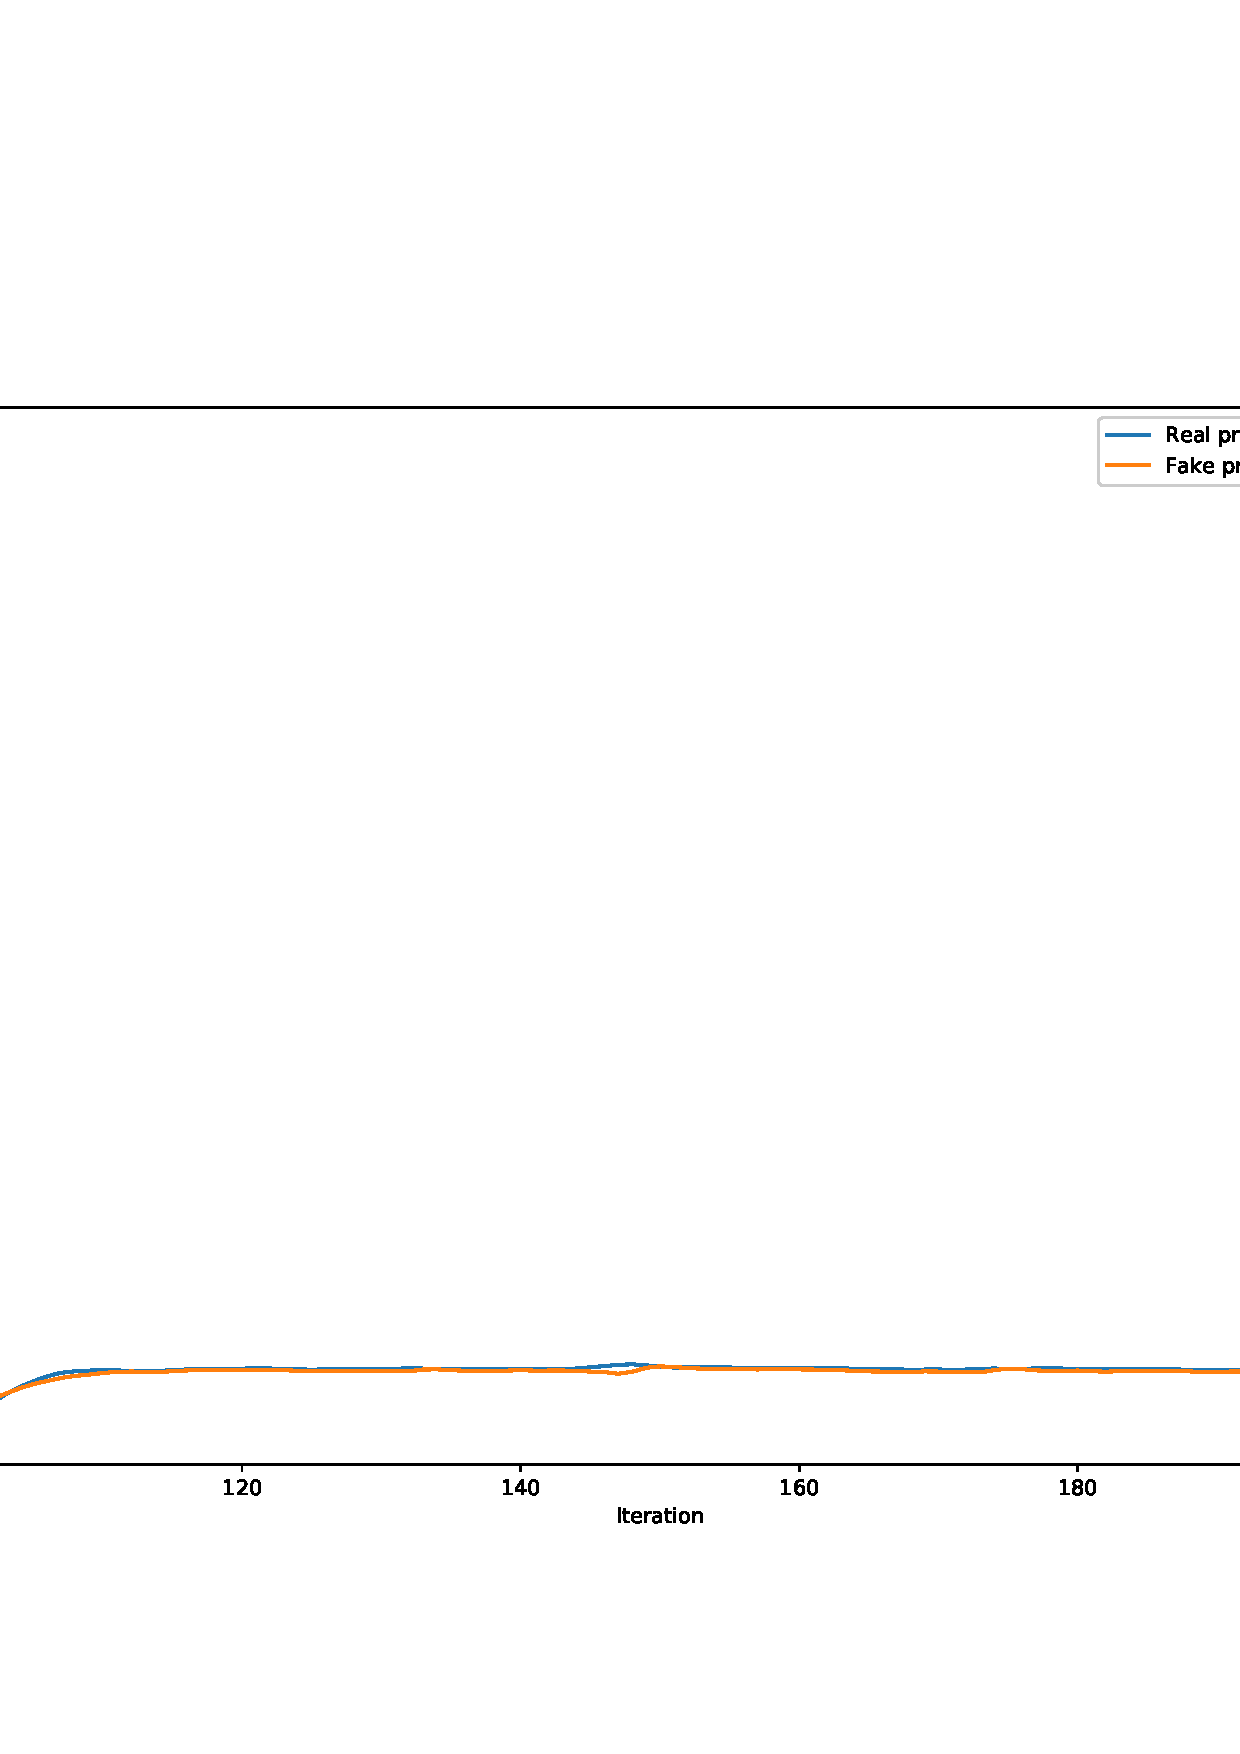
\includegraphics[width=\textwidth]{results/freezeInDG1.png}
%        \caption{Weight freezing in old layers}
%        \label{fig:freezeInDG1}
%    \end{subfigure}
%    \begin{subfigure}[b]{0.45\textwidth}
%        \includegraphics[width=\textwidth]{results/fadeInDG1.png}
%        \caption{Fade in new layers}
%        \label{fig:freezeInDG2}
%    \end{subfigure}
%    \caption{Discriminator output on real and fake images during transition between 16x16 and 32x32 resolution images for the different transition strategies.}
%    \label{fig:fadeVsFreeze}
%\end{figure}


\section{Autoencoding \acrshort{gans}}
The final method tested in this project is based on a combination of autoencoders and \acrshort{gans}. The proposed method consists of simultaneuously training a denoising autoencoder and a \acrshort{gan}, using the same network as generator and decoder. The idea is conceptually similar to the VAEGAN framework \parencite{LarsenSW15autoencodingbeyond}. There are two major differences between this method and the VAEGAN framework, first and foremost the autoencoder trained in this method is deterministic and trained with the mean squared error loss functions. Secondly, the adversarial loss is not used to train the autoencoder, instead a normal GAN is trained separately form the autoencoder but with the decoder network as the generator. 

Given enough capacity in the generator and encoder, the global minimum for the autoencoder training in this setting corresponds to the autoencoder learning the identity mapping. This causes the generator to generate realistic images on the points in the latent space the autoencoder maps the original data onto. The optimal generator in the \acrshort{gan} framework maps the entire latent space to realistic images. From this point of view the two objectives should lead to the same solution, however \acrshort{gans} tend to suffer from mode collapse and autoencoders often produce poor samples in terms of visual quality. In case of convergence this method should enforce the decoded images to be sharp and the generator to capture the entire training data distribution.
% Idé till presentationen: "Variational autoencoders are stable and good at ...blablabla... . On the other hand there are two major problems with variational autoencoders, 1: they are variational (Åtgärda KL-term), 2: they are autoencoders (pixel-loss ersätts med GANs)."


